\documentclass[border=3pt, tikz, convert]{standalone}

\usepackage{pgf}
\usepackage{tikz}
\usetikzlibrary{arrows,automata}
\usepackage[latin1]{inputenc}
\begin{document}


% Directed graph
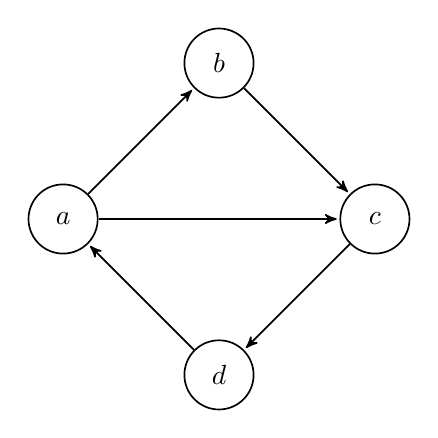
\begin{tikzpicture}[->,>=stealth',shorten >=1pt,auto,node distance=2.8cm,
                    semithick]
  \tikzstyle{every state}=[draw=black,text=black]

  \node[state]         (A)                    {$a$};
  \node[state]         (B) [above right of=A] {$b$};
  \node[state]         (D) [below right of=A] {$d$};
  \node[state]         (C) [below right of=B] {$c$};

  \path (A) edge node {} (B)
            edge node {} (C)
        (B) edge node {} (C)
        (C) edge node {} (D)
        (D) edge node {} (A);
\end{tikzpicture}

% undirected graph
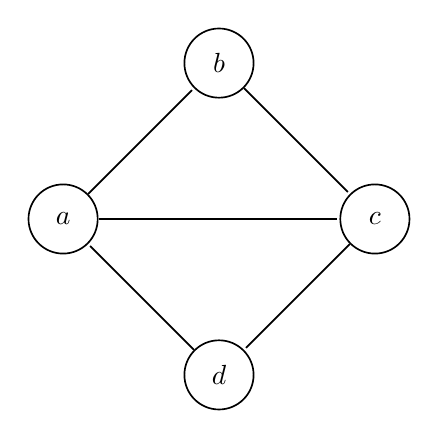
\begin{tikzpicture}[>=stealth',shorten >=1pt,auto,node distance=2.8cm,
                    semithick]
  \tikzstyle{every state}=[draw=black,text=black]

  \node[state]         (A)                    {$a$};
  \node[state]         (B) [above right of=A] {$b$};
  \node[state]         (D) [below right of=A] {$d$};
  \node[state]         (C) [below right of=B] {$c$};

  \path (A) edge node {} (B)
            edge node {} (C)
        (B) edge node {} (C)
        (C) edge node {} (D)
        (D) edge node {} (A);
\end{tikzpicture}

% weighted undirected graph
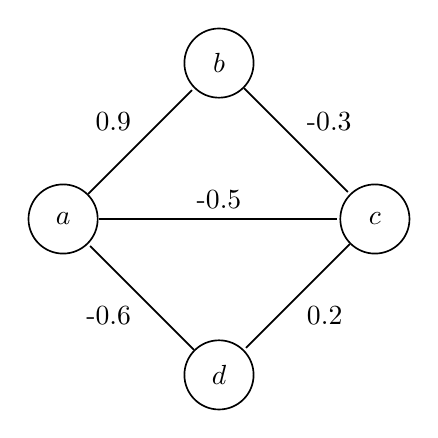
\begin{tikzpicture}[>=stealth',shorten >=1pt,auto,node distance=2.8cm,
                    semithick]
  \tikzstyle{every state}=[draw=black,text=black]

  \node[state]         (A)                    {$a$};
  \node[state]         (B) [above right of=A] {$b$};
  \node[state]         (D) [below right of=A] {$d$};
  \node[state]         (C) [below right of=B] {$c$};

  \path (A) edge node {0.9} (B)
            edge node {-0.5} (C)
        (B) edge node {-0.3} (C)
        (C) edge node {0.2} (D)
        (D) edge node {-0.6} (A);
\end{tikzpicture}

\end{document}